\documentclass[12pt]{letter}
\usepackage{amsmath,amsfonts,amsthm,amstext,amssymb,graphicx, multicol,fancyhdr,lastpage,fullpage,framed,fancybox,enumerate,tikz,color,mathrsfs, polynom}
\usepackage[margin=0.6in,headsep=3pt, headheight=15pt]{geometry}

% ----------------------------------------------------------
% Custom Definitions, Commands, Environments, etc.

% Sets of numbers
\def\R{\mathbb{R}} % The reals
\def\N{\mathbb{N}} % The naturals
\def\Z{\mathbb{Z}} % The integers
\def\Q{\mathbb{Q}} % The rationals

% Blank space
\newcommand{\blank}[1]{\underline{\hspace{#1}}} % Blank space

% Change font colors
\newcommand{\cyan}[1]{{\color{cyan}{#1}}} % Changes font to cyan
\newcommand{\red}[1]{{\color{red}{#1}}} % Changes font to red
\newcommand{\magenta}[1]{{\color{magenta}{#1}}} % Changes font to magenta
\newcommand{\orange}[1]{{\color{orange}{#1}}} % Changes font to orange
\newcommand{\yellow}[1]{{\color{yellow}{#1}}} % Changes font to yellow
\newcommand{\violet}[1]{{\color{violet}{#1}}} % Changes font to violet
\newcommand{\green}[1]{{\color{green}{#1}}} % Changes font to green
\newcommand{\blue}[1]{{\color{blue}{#1}}} % Changes font to blue
\newcommand{\white}[1]{{\color{white}{#1}}} % Changes font to white

% Fitted inclusion symbols
\newcommand{\fp}[1]{\left({#1}\right)} % Fitted parentheses around content
\newcommand{\fb}[1]{\left[{#1}\right]} % Fitted brackets
\newcommand{\set}[1]{\left\{{#1}\right\}} % Fitted braces (useful for sets)
\newcommand{\av}[1]{\left|{#1}\right|} % Fitted absolute value bars

% Augmented Matrix Environment
\newenvironment{amatrix}[1]{%
	\left[\begin{array}{@{}*{#1}{c}|c@{}}
	}{%
	\end{array}\right]
}

% Miscellaneous
\def\then{\Rightarrow}
\def\to{\rightarrow}
\def\d{^{\circ}}
\newcommand{\?}{\stackrel{?}{=}}



% Coordinate Plane (Four-Quadrant)
\def\coordplane {
	\begin{tikzpicture}		\draw[step=0.25cm,black,very thin,opacity=0.25] (-2.5cm, -2.5cm) grid (2.5cm, 2.5cm);
	\draw[<->,thick,black] (-2.5cm, 0) -- (2.5cm, 0) node[anchor=north west,pos=0.94,font=\scriptsize]{$x$};
	\draw[<->,thick,black] (0,-2.5cm) -- (0, 2.5cm) node[anchor=south east,font=\scriptsize,pos=0.94]{$y$};
	\end{tikzpicture}
}

% Coordinate Plane (One-Quadrant)
\def\onequad {
	\begin{tikzpicture}
	\draw[step=0.25cm, black, very thin, opacity=0.25] (0,0) grid (7.5cm,5cm);
	\draw[->, thick, black] (0,0) -- (7.5cm, 0) node[anchor=north west,font=\scriptsize,pos=0.94]{$x$};
	\draw[->, black, thick] (0,0) -- (0,5cm) node[anchor=south east,font=\scriptsize,pos=0.94]{$y$};
	\end{tikzpicture}
}

% Counters
\newcounter{exercise}

% Exercise environment (auto-numbered)
\newenvironment{exercise}[1][]{\begin{framed}\refstepcounter{exercise}\textbf{Exercise~\theexercise:} #1}{\end{framed}}

% Book exercise environment
\newenvironment{bex}[2][] {
	\begin{framed}
		\textbf{Book Exercise {#2}}#1
	\end{framed}
}
% ----------------------------------------------------------

% ----------------------------------------------------------
% Header and Footer Information
% \pagestyle{fancy}
% \fancyhf{}
% \renewcommand{\headrulewidth}{0pt}
% \rhead{Name: \blank{2in}}
% \lhead{@}
% \rfoot{Page \thepage \, of \,\pageref{LastPage}}
% ----------------------------------------------------------
\author{Jacob Ayers}

\begin{document}
	\textbf{Assignment 9 Key \\ MAT 130}
	
	\begin{bex}{5.2.10}
		{
			
		}
	\end{bex} \vspace{-8pt}
	
	% My answer here
	$32^{2/5} = 4$
	
	\vfill % \newpage
	
	\begin{bex}{5.2.12}
		{
			
		}
	\end{bex} \vspace{-8pt}
	
	% My answer here
	$\log_9 27 = \dfrac32$
	
	\vfill % \newpage
	
	\begin{bex}{5.2.16}
		{
			
		}
	\end{bex} \vspace{-8pt}
	
	% My answer here
	$\log_{25} 5 = \dfrac12$
	
	\vfill % \newpage
	
	\begin{bex}{5.2.18}
		{
			
		}
	\end{bex} \vspace{-8pt}
	
	% My answer here
	$\log 10 = 1$
	
	\vfill % \newpage
	
	\begin{bex}{5.2.24}
		{
			
		}
	\end{bex} \vspace{-8pt}
	
	% My answer here
	$\log 96.75 \approx 1.986$
	
	\vfill % \newpage
	
	\begin{bex}{5.2.26}
		{
			
		}
	\end{bex} \vspace{-8pt}
	
	% My answer here
	$\log_\pi \pi^2 = 2$
	
	\vfill % \newpage
	
	\begin{bex}{5.2.28}
		{
			
		}
	\end{bex} \vspace{-8pt}
	
	% My answer here
	$5^{\log_5 3} = 3$
	
	\vfill % \newpage
	
	\begin{bex}{5.2.30}
		{
			
		}
	\end{bex} \vspace{-8pt}
	
	% My answer here
	$x - 3 = 9 \then x = 12$
	
	\vfill % \newpage
	
	\begin{bex}{5.2.32}
		{
			
		}
	\end{bex} \vspace{-32pt}
	
	% My answer here
	\begin{flalign*}
	x^2 + 6x &= 27 & \\
	x^2 + 6x - 27 &= 0 & \\
	(x + 9)(x - 3) &= 0 & \\
	x &= \set{-9, 3}
	\end{flalign*}
	
	\vfill \newpage
	
	\begin{bex}{5.2.42}
		{
			
		}
	\end{bex} \vspace{-8pt}
	
	% My answer here
	Domain: $x > 0$ \\ $x$-intercept: $(1, 0)$ \\ Vertical asymptote at $x = 0$
	
	
	\begin{tabular}{c|cccc}
		$x$ & 1 & 6 & 36 & 216 \\ \hline
		$g(x)$ & 0 & 1 & 2 & 3
	\end{tabular}

	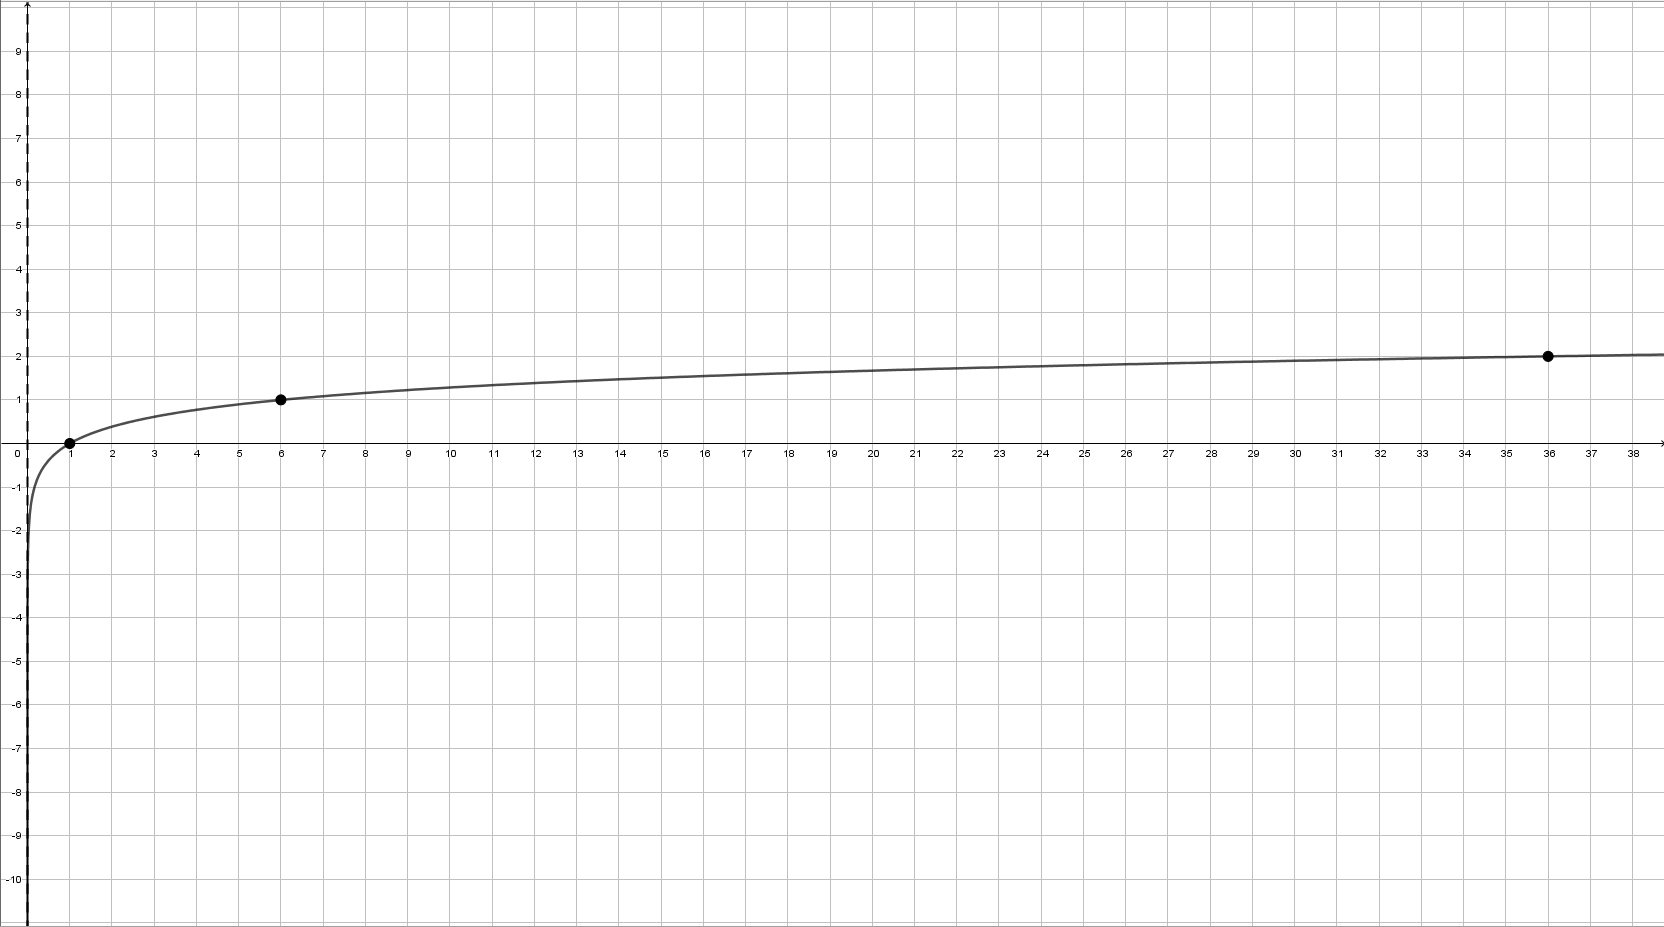
\includegraphics[width=3in]{5242.png}
	
	\vfill % \newpage
	
	\begin{bex}{5.2.58}
		{
			
		}
	\end{bex} \vspace{-8pt}
	
	% My answer here
	$3 \ln 0.74 \approx -0.903$
	
	\vfill \newpage
	
	\begin{bex}{5.2.80}
		{
			
		}
	\end{bex} \vspace{-8pt}
	
	% My answer here
	(a) We need to evaluate $P(8)$ and $P(12)$. I used a graphing calculator to find these values:
	
	\begin{tabular}{c|cc}
		Year & 2008 & 2012 \\ \hline
		Percentage & $18.156$ & $35.255$
	\end{tabular}

	(b) 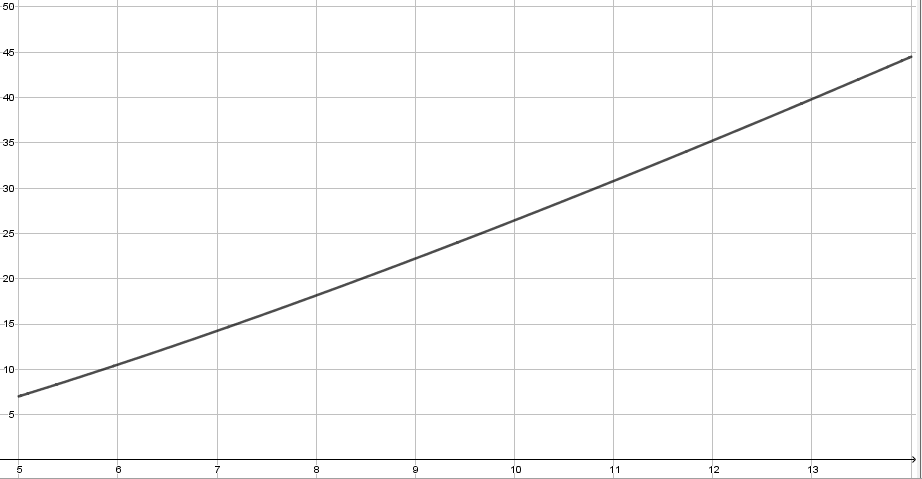
\includegraphics[width=3in]{5280b.png}
	
	(c) Neither 2020 nor 2030 is in the domain of the model, so there is reason for skepticism, but perhaps the model can be extended beyond its original time frame. To see if it is reasonable to use this model to predict the percentage of households with wireless telephone service in 2020 and 2030, we should evaluate the function at $t = 20$ and $t = 30$ and see if the result is reasonable.
	
	\begin{tabular}{c|cc}
		Year & 2020 & 2030 \\ \hline
		Percentage & $74.289$ & $128.92$
	\end{tabular}

	A prediction that about 75\% of households will have wireless-only service in 2020 seems reasonable (if not a bit low), but it is impossible for over 100\% of the population to have the service, so the model does not give a reasonable prediction for 2030.
	
	\vfill \newpage
	
	\begin{bex}{5.2.83}
		{
			
		}
	\end{bex} \vspace{-8pt}
	
	% My answer here
	(a) 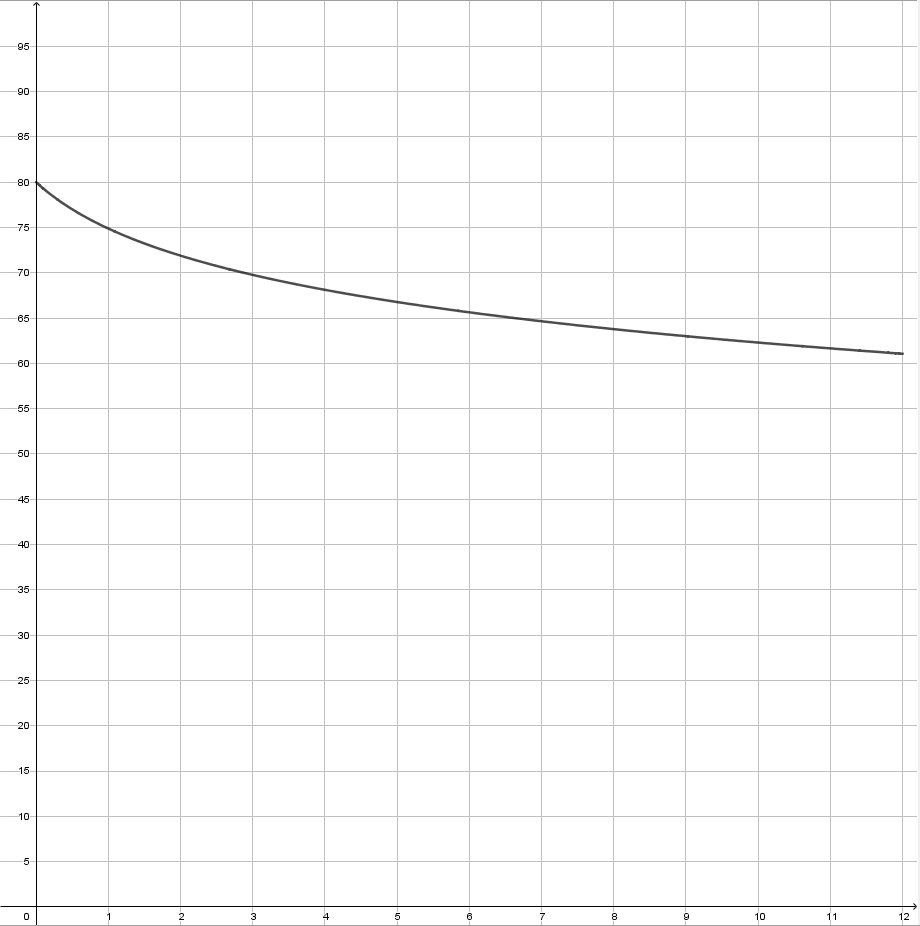
\includegraphics[width=3in]{5283a.png}
	
	(b-d) Using a graphing calculator:
	
	\begin{tabular}{c|ccc}
		Time (months) & 0 & 4 & 10 \\ \hline
		Average Score & 80 & 68.118 & 62.296
	\end{tabular}
	
	\vfill % \newpage
	
	\begin{bex}{5.3.10}
		{
			
		}
	\end{bex} \vspace{-8pt}
	
	% My answer here
	$\log_{0.4} 12 = \dfrac{\log 12}{\log 0.4} \approx -2.712$
	
	\vfill % \newpage
	
	\begin{bex}{5.3.12}
		{
			
		}
	\end{bex} \vspace{-8pt}
	
	% My answer here
	$\log_{2/3} 0.125 = \dfrac{\log 0.125}{\log(2/3)} \approx 5.129$
	
	\vfill % \newpage
	
	\begin{bex}{5.3.16}
		{
			
		}
	\end{bex} \vspace{-8pt}
	
	% My answer here
	Note that the prime factorization of $175$ is $5^2 \cdot 7$. Thus \begin{flalign*}
	\log_3 125 &= \log_3 \fp{5^2 \cdot 7} & \\
	&= \log_3 5^2 + \log_3 7 & \\
	&= 2\log_3 5 + \log_3 7
	\end{flalign*}
	
	\vfill \newpage
	
	\begin{bex}{5.3.22}
		{
			
		}
	\end{bex} \vspace{-8pt}
	
	% My answer here
	Note that $\sqrt[4]{8} = \sqrt[4]{2^3} = 2^{3/4}$. Thus
	
	$\log_2 \sqrt[4]{8} = \log_2 2^{3/4} = \dfrac34$
	
	\vfill % \newpage
	
	\begin{bex}{5.3.34}
		{
			
		}
	\end{bex} \vspace{-8pt}
	
	% My answer here
	$\log_b 2 \approx 0.3562$, $\log_b 3 \approx 0.5646$ \begin{flalign*}
	\log_b \dfrac23 &= \log_b 2 - \log_b 3 & \\
	&\approx 0.3562 - 0.5646 & \\
	&\approx -0.2084
	\end{flalign*}
	
	\vfill % \newpage
	
	\begin{bex}{5.3.36}
		{
			
		}
	\end{bex} \vspace{-8pt}
	
	% My answer here
	$\log_b 2 \approx 0.3562$ \begin{flalign*}
	\log_b \sqrt{2} &= \log_b 2^{1/2} & \\
	&= \dfrac12 \log_b 2 & \\
	&\approx \dfrac12\fp{0.3562} & \\
	&\approx 0.1781
	\end{flalign*}
	
	\vfill % \newpage
	
	\begin{bex}{5.3.42}
		{
			
		}
	\end{bex} \vspace{-8pt}
	
	% My answer here
	$\log_3 13z = \log_3 13 + \log_3 z$
	
	\vfill % \newpage
	
	\begin{bex}{5.3.46}
		{
			
		}
	\end{bex} \vspace{-32pt}
	
	% My answer here
	\begin{flalign*}
	\log_6 \dfrac{w^2}{v} &= \log_6 w^2 - \log_6 v & \\
	&= 2\log_6 w - \log_6 v
	\end{flalign*}
	
	\vfill % \newpage
	
	\begin{bex}{5.3.50}
		{
			
		}
	\end{bex} \vspace{-32pt}
	
	% My answer here
	\begin{flalign*}
	\log_4 11b^2 c &= \log_4 11 + \log_4 b^2 + \log_4 c & \\
	&= \log_4 11 + 2 \log_4 b + \log_4 c
	\end{flalign*}
	
	\vfill \newpage
	
	\begin{bex}{5.3.62}
		{
			
		}
	\end{bex} \vspace{-8pt}
	
	% My answer here
	$\log_5 8 - \log_5 t = \log_5 \dfrac{8}{t}$
	
	\vfill % \newpage
	
	\begin{bex}{5.3.66}
		{
			
		}
	\end{bex} \vspace{-32pt}
	
	% My answer here
	\begin{flalign*}
	2\log_2 x + 4\log_2 y &= \log_2 x^2 + \log_2 y^4 & \\
	&= \log_2 x^2y^4
	\end{flalign*}
	
	\vfill % \newpage
	
	\begin{bex}{5.3.70}
		{
			
		}
	\end{bex} \vspace{-32pt}
	
	% My answer here
	\begin{flalign*}
	3\log_3 x + \dfrac14 \log_3 y - 4\log_3 z &= \log_3 x^3 + \log_3 y^{1/4} - \log_3 z^4 & \\
	&= \log_3 \dfrac{x^3y^{1/4}}{z^4} & \\
	&= \log_3 \dfrac{x^3\sqrt[4]{y}}{z^4}
	\end{flalign*}
	
	\vfill % \newpage
	
	
	
\end{document}